\documentclass[tikz,border=2pt]{standalone}
\usepackage{amsmath,amssymb}
\usepackage{tikz}
\usetikzlibrary{arrows.meta}

\begin{document}
% Two linear constraints in the plane: independent rows (normals not parallel) meet in a single
% point and cut the dimension by 2; dependent rows describe the same (or parallel) lines and
% remove only one dimension — or nothing feasible at all.
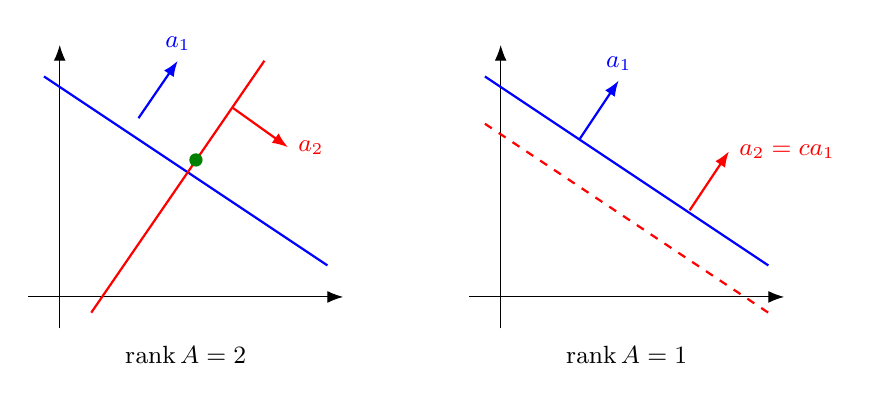
\begin{tikzpicture}[every node/.style={font=\small}, >={Latex[length=2mm]}]
	\begin{scope}
		\draw[->] (-0.4,0) -- (3.6,0); \draw[->] (0,-0.4) -- (0,3.2);
		\draw[blue, thick] (-0.2,2.8) -- (3.4,0.4);
		\draw[red, thick] (0.4,-0.2) -- (2.6,3.0);
		\fill[green!50!black] (1.73,1.74) circle (2.4pt);
		\draw[->, blue, thick] (1.0,2.27) -- (1.5,3.0) node[above] {$a_1$};
		\draw[->, red, thick] (2.2,2.4) -- (2.9,1.9) node[right] {$a_2$};
		\node[anchor=north] at (1.6,-0.5) {$\operatorname{rank}A=2$};
	\end{scope}
	\begin{scope}[xshift=5.6cm]
		\draw[->] (-0.4,0) -- (3.6,0); \draw[->] (0,-0.4) -- (0,3.2);
		\draw[blue, thick] (-0.2,2.8) -- (3.4,0.4);
		\draw[red, thick, dashed] (-0.2,2.2) -- (3.4,-0.2);
		\draw[->, blue, thick] (1.0,2.0) -- (1.5,2.75) node[above] {$a_1$};
		\draw[->, red, thick] (2.4,1.1) -- (2.9,1.85) node[right] {$a_2=ca_1$};
		\node[anchor=north] at (1.6,-0.5) {$\operatorname{rank}A=1$};
	\end{scope}
\end{tikzpicture}
\end{document}
